Our data on Soviet repressions come from  the Victims of Political Terror in the USSR database by the Russian human rights organization \citet{memorial_zhertvy_2017}.\footnote{The database can be accessed and searched from  \url{http://base.memo.ru/} (new version) or at \url{http://lists.memo.ru/} (older version). However, we downloaded the file with every record from the database from \url{https://github.com/MemorialInternational/memorial_data_FULL_DB/blob/master/data/lists.memo.ru-disk/lists.memo.ru-disk.zip}} 
The Memorial data has already been used in empirical research by \citet{zhukov_stalins_2018} to estimate the  effects of the Soviet repressions on the current political participation. 
 The main sources of the Memorial lists are declassified Russian Interior Ministry documents, prosecutor’s offices and the Commission for the Rehabilitation of Victims of Political Repression, and \enquote{Books of Memory}. 
Vast  majority records in the database are individual arrests under  Article 58. 
This means that the victims of other repressive activities of the Soviet state such mass forced migration, counter-insurgency operations of the Red Army during Russian Civil War or famines are mostly excluded. Therefore our research focuses on one  particular type of repression (individual arrests by the NKVD). 

Nevertheless, even if we restrict ourselves to the individual arrests, the Memorial database is still not complete.
According to some estimates

At the time of our access to the database, the database contained 2.7 million records which is approximately 70\% of estimated 3.8 million people convicted under Article 58 between 1921 and 1953 \citep{zhukov_stalins_2018}.

%\footnote{In particular, we downloaded the data from the replications file archive of the journal available  from \url{https://www.prio.org/JPR/Datasets/}} who use  the Victims of Political Terror archive  collected by a Russian NGO Memorial.
%individual arrests by the Soviet secret police (NKVD) between  the years 1921 and 1959 with names of each person, date of arrest, the place of birth for all observations and  in many cases additional information such as ethnicity, occupation and party membership. 
 %However, the data are not complete and include only about 70\% of estimated 3.8  million people convicted under Article 58.

%Another major issue with the data is frequent  missingness of information on ethnicity and date of arrests. 
%We try to address this issue by imputing missing values using names and date of process. The imputation procedures are described in section \ref{subsec:inferring_ethnicity} \ref{subsec:imputing_missing_date}.

%\subsection{Missing Data Analysis}
Missing data presents another major challenge. 
%Another major issue with the data is frequent  
 Table \ref{tab:missing_data_count} shows how many values are missing for the variables of our interest. We can see that information on ethnicity is not available for more than half of all observations. In contrast, a surname is recorded for every arrest in the dataset and a first name is missing only for negligible fraction of observations. The availability of information on names enables us to use them to infer missing ethnicity of an individual. In particular, we will train a Naive Bayes classifier on the \mbox{1 197 373} observations with known ethnicity and use the model's predictions to impute the ethnicity for the remaining 1 507 177 observations (the details are described in the subsection \ref{subsec:inferring_ethnicity}).
\begin{table}[t]

\caption{\label{tab:missing_data_count}Missing Data by Variable}
\centering
\begin{tabular}{lrr}
\toprule
Variable & Number of Missing Obs. & Percent of Missing Obs.\\
\midrule
Ethnicity & 1 507 177 & 55.73\\
Date of Arrest & 1 650 912 & 61.04\\
Date of Process & 943 108 & 34.87\\
First Name & 14 006 & 0.52\\
\bottomrule
\end{tabular}
\end{table}

Date of arrest, which is also necessary for our analysis, has even higher rate of missingness than ethnicity.\footnote{
We consider a date missing only if not even year of arrest is available. Many observations have information on year of arrest even though the exact month or day are missing. We do not categorize these observation as having missing date of arrest since our fundamental unit of analysis is a year and thus month and day are not of high interest to us. The same applies to the date of trial.} 
One solution, albeit only partial, might be to use the date of trial    to extrapolate the missing date of arrest where the trial date is available.
As is shown in the table \ref{tab:missing_date_of_arrest_process}, we could impute this way the missing date of arrests for 903 493 observations for which we have the date of trial. 
Total number of arrests used for our analysis would therefore increase from 1 053 638 to  1 957 131.  However, there remains 747 419 observations for which neither the date of arrest nor the date of trail are known. 
Unfortunately, not much can be done address this problem.
%The table \ref{tab:missing_date_of_arrest_process} shows for this 
\begin{table}[t]

\caption{\label{tab:missing_date_of_arrest_process}Missing Dates of Arrest and Process}
\centering
\begin{tabular}{lrr}
\toprule
\multicolumn{1}{c}{ } & \multicolumn{2}{c}{Date of Arrest} \\
\cmidrule(l{2pt}r{2pt}){2-3}
Date of Process & Missing & Present\\
\midrule
Missing & 747 419 & 195 689\\
Present & 903 493 & 857 949\\
\bottomrule
\end{tabular}
\end{table}
%\begin{table}[t]

\caption{\label{tab:missingness_of_ethnicity_and_date}Missingness of Ethnicity and Dates of Arrest and Trial}
\centering
\begin{tabular}{lrr}
\toprule
\multicolumn{1}{c}{ } & \multicolumn{2}{c}{Date of Arrest or Trial} \\
\cmidrule(l{2pt}r{2pt}){2-3}
Ethnicity & Missing & Present\\
\midrule
Missing & 594 975 & 912 202\\
Present & 152 444 & 1 044 929\\
\bottomrule
\end{tabular}
\end{table}

%When we consider only the data with non-missing
%The original Memorial data has 
There are more than 100 different ethnicities in the Memorial data. 
However, in many cases there are no more than hundred of people in the whole database that belong to a given ethnic groups. 
%Furthermore, in a f
%Moreover, it appears that 
%This would present problem for the  imputation of missing ethnicity since our model would not have enough data to train on. 
Therefore we decided to limit ourselves only to ethnic groups with at least 900 individuals in the Memorial database. 
This leaves us with 38 ethnic groups. 
%many of them are represented by less than  

%Chechen 953
%Uyghur 851

After imputations of ethnicity and the date of arrest had been applied,  we created our main dataset by counting number of arrest for each ethnicity by year. %In the original dataset, there were more than 120 different ethnicities. Some of them however have very low frequency and thus
%A few people who were categorized as having multiple ethnicities were dropped from the dataset and not counted. 
With 38  ethnic groups  and 40 time periods (from 1921 to 1960), we have 1520 observations in total. Basic descriptive statistics  for each ethnicity are provided in the table \ref{tab:descr_stats_by_ethnicity}.  The plot of arrest by ethnicity and year (after applying the transformation $\log\left(1 + y_{it}\right)$) is shown in figure \ref{fig:facet_by_year}. 

In addition to data on repressions, we also obtained some information on some characteristics of the  ethnic groups in our dataset that we will use as covariates in the synthetic control method. 
In particular, we acquired total population of the ethnic groups and their urbanization rate from 1926 Soviet Census from the Demoscope website.\footnote{It is available online at \url{http://www.demoscope.ru/weekly/ssp/ussr_nac_26.php}} For each ethnic group, we also calculated the cladisitc similarity of its language to Russian based from Glottolog language trees \citep{hammarstrom_glottolog_2018}.
Cladistic measure of linguistic similarity counts the number of shared branching points between the two nodes on a language tree. It has been used by \citet{fearon_ethnic_2003} and \citet{dickens_ethnolinguistic_2018} among others. 
%For example, Ukrainian and Russian have the cladisitc similarity of 4 since they are both
The full data are provided in the table \ref{tab:sc_predictors} in the appendix.


\newpage
\section{Imputation of Missing Data} \label{sec:missing_data}
%napis o missing at random, completely at random asumptions
\subsection{Inferring Ethnicity from Names} \label{subsec:inferring_ethnicity}
In this section, we explain our method for predicting ethnicity of an individual from his or her names. Using names for imputing ethnicity has several advantages. First, full name  is available for every individuals in the dataset. Second, names have been shown to be highly predictive of ethnicity in a variety of applications \citep{mateos_review_2007, hofstra_sources_2017, hofstra_predicting_2018}. 
%Finally, it seems 

Given the high number of predictors, we need a model that is not  computationally demanding but at the same time achieves reasonable level of prediction accuracy. Naive Bayes classifier meets these criteria and has been for this reason used in wide range of applications including text classification  \citep{gentzkow_text_2019}.
%We will brief introduce its 

\subsubsection{Naive Bayes Classifier}
%In particular, we use Naive Bayes classifier. 
Let  $\boldsymbol{x} = \left(x_1, x_2, x_3\right)$ be features used for predicting ethnicity, that is a person's first, last, and patronymic (given after father's first name) names. Using Bayes theorem, we can express the probability that particular observation  belongs to ethnic group $E_k$ given its features as
\begin{equation}
p(E_k \mid \mathbf{x}) = \frac{p(E_k) \ p(\mathbf{x} \mid E_k)}{p(\mathbf{x})},
\end{equation}
in other words, the posterior probability is proportional to the product of prior probability and likelihood. 
Assuming conditional independence of features allows us to substitute $p(\mathbf{x} \mid E_k)$ such that we get

\begin{equation}
p(E_k \mid \mathbf{x}) = \frac{p(E_k) \  \prod_{i=1}^3 p(x_i \mid E_k)\,}{p(\mathbf{x})}.
\end{equation}
%In this context, the conditional independence of features means within each ethnic group having a certain first name does not influence probability of having some surnames and patronymic names   
 All terms in this equation now can be estimated from the data: the prior probability $p(E_k)$ as a proportion of $E_k$ in the data, $p(x_i \mid E_k)$ as a proportion of people with name $x_i$ in the ethnic group $E_k$ and $p(\mathbf{x})$ simply calculated such that the sum of $p(E_k \mid \mathbf{x})$ for all $k$ is one. 
%Thus, having a name that is typical for a given ethnicity results in high probabilty
%The Naive Bayes classifier assigns high probability to names that are 
The Naive Bayes classifier then chooses the ethnicity with the highest posterior probability as its prediction, that is
\begin{equation}
    \hat{y} = \underset{k \in \{1, \dots, K\}}{\operatorname{argmax}} \ p(E_k) \displaystyle\prod_{i=1}^{3} p(x_i \mid E_k).
\end{equation}

However, one potential issue is that whenever a likelihood of a certain feature is estimated to be 0 then the posterior probability is always 0 regardless of the prior  or the likelihoods of other features. For example, suppose that a person has a typical German first name but a rare surname which does not appear in the training set at all. 
Then the useful information contained in the first name will be completely ignored since the zero likelihood of the surname will override any other value and we will end up with the posterior probability of zero for all ethnic groups.

To address this problem, we apply Laplace smoothing. 
For every ethnicity, let $c_j$ be number of people with a name $j$ and $N$ be total number of member of that ethnic group in the data.  Without applying any smoothing, we would estimate the likelihood  $p(x_i \mid E_k)$ simply as a relative frequency, i.e. $\hat\theta_j = \frac{c_j}{N}$. With  Laplace smoothing, we estimate  the  likelihood $\hat\theta_j$ as 
\begin{equation}
    \hat\theta_j = \frac{c_j + \alpha}{N + \alpha d} \qquad j = 1, \dots, d
\end{equation}
where parameter $\alpha > 0 $ is a smoothing parameter.  This ensures that for any finite value of $N$,  $\hat\theta_j$ will never be zero. %Nevertheless,  $\alpha$ should not be set too high since that could 
In our model, relatively small value of  $\alpha = 0.005 $  turned out to be sufficient and  was chosen. 

It is important to note that the conditional independence assumption often does not hold in the data and the estimated posterior probabilities therefore have to be taken with a grain of salt. %have are thus not always reliable. 
However, our main goal is the best out-of-sample accuracy of the model's predictions. In this respect, Naive Bayes classifier have been shown to perform  well in many applications, despite its often violated assumptions \citep{domingos_optimality_1997}.

\subsubsection{Adjusting for Unbalanced Prediction Accuracy} \label{subsubsec:pred_adj}
To reliably asses the out-of-sample performance of our model, we used 10-fold cross-validation on the data with non-missing ethnicity. That is, the data is first randomly split into 10 groups. A model is fitted to 9 group and the remaining group is used to test the model's performance. This process is then repeated 9 times  until every group has been tested. 
Using this method, the resulting overall accuracy of our model is 78.7\%. However,  we are also interested how it varies by ethnicity.
For this reason we calculate sensitivity and specificity for each ethnic group.\footnote{Sensitivity measures the proportion of observations in the class that are correctly identified by the model as such (i.e. number of true positives divided by all positives). Specificity measures the proportion of observations \emph{not} in the class that are correctly identified as such (i.e. number of true negatives divided by all negatives).} 
The results, provided in the table \ref{tab:sens_spec} in the appendix, show that the sensitivity differs significantly by ethnicity. 
Some ethnic groups with distinctive names such as Chinese or Japanese are classified  with accuracy higher than 95\%  while for other ethnicities such as Chuvash or Udmurt it is about 10\%. This severe imbalance in sensitivity and specificity  across ethnic groups could potentially cause bias in the imputations. 

Therefore we develop adjustments that try to correct for these biases in the model's predictions. Let $P_{it}$ be the number of people with predicted ethnicity $i$ arrested at time $t$, $R_{it}$ be actual the number of people with ethnicity $i$ arrested at time $t$, $\alpha_i$ and $\beta_i$  be sensitivity and specificity of our classifier for ethnic group $i$ and $N_t$ be the total number of arrests at time $t$. Then the predicted arrests of a given ethnicity are sum of true positives and false positives, that is
\begin{equation}
    P_{it} = \alpha_i R_{it} + \left( N_t - R_{it} \right) \cdot \left(1 - \beta_i \right).  
\end{equation}
We are interested in $R_{it}$ but we only directly observe $P_{it}$ and $N_t$. However using simple algebra, $R_{it}$ can be expressed as
\begin{equation} \label{eq:pars_adj}
 R_{it} = \frac{P_{it} - N_t  \left(1 - \beta_i \right)}{\alpha_i + \beta_i - 1}.
\end{equation}
We will refer to this method of correcting predictions as parsimonious adjustment.  The parameters $\alpha_i$ and $\beta_i$ are not known to us but we can use their estimates from the cross-validation on the training data. This assumes that the these parameters do not differ significantly for the training and test data. But this might not be the case. 
Suppose, for example, that Armenians are often misclassified as Chechens and that the number of Armenians in the data with missing ethnicity  is disproportionately higher than in the data with information on ethnicity. 
Then the cross-validated specificity for Chechens in the training set will underestimate the specificity in the test set because it does not take into account higher proportion of Armenians. 
%If, for example, the proportions of the arrests of some ethnic group are substantially different between the test and training set and if there is constant then 

Fortunately, we can address this potential bias by more building complex modeling.
First for all ethnic groups $i$ and $j$, we define the misclassification rate $b_{ij}$ as share of people with ethnicity $j$ that are classified as $i$.
Notice that for $i = j$, the misclassification rate is simply prediction accuracy for ethnicity $i$.
It follows from the definition of the terms that predicted number of arrests for ethnic group $i$ at time $t$,  $P_{it}$, is equal to 
\begin{equation}
P_{it}  = \sum_{j = 1}^{K} b_{ij} R_{jt} \qquad i = 1, \dots, K.
\end{equation}
This equation can be expressed in matrix form as
\begin{equation}
 \mathbf{P}_t = \mathbf{B} \cdot \mathbf{R}_t,
\end{equation}
where $\mathbf{P}_t = \left(P_{1t}, \cdots, P_{Kt} \right)$, $\mathbf{R}_t = \left(R_{1t}, \cdots, R_{Kt} \right)$, and $\mathbf{B} = \left(b_{ij}\right)_{i = 1, \dots, K,\:j = 1, \dots, K}$.
To express $\mathbf{R}_t$, we just  apply basic linear algebra
\begin{equation} \label{eq:full_matrix_adj}
\mathbf{R}_t  = \mathbf{B}^{-1} \cdot  \mathbf{P}_t.
\end{equation}
We will call this method the full matrix adjustment. Compared to the parsimonious adjustment (in equation \ref{eq:pars_adj}), this correction no longer assumes that the test set sensitivity and specificity be accurately estimated  from the training set.  The full matrix adjustment
makes only somewhat weaker assumption that the train and test set misclassification rates are not significantly different. 
%On the other hand, it might be noisier
% lower bias, higher variance

One issue that we encountered when applying these adjustments was that some values of $\mathbf{R}_t$ were negative. Thus, we replaced all negative values with zero. Finally, we scaled all  the values such that the total number of arrests would stay unchanged after the adjustment and rounded it to the nearest integer. The results 

% Jeste se zmin o scalovani

%\begin{equation*}
%\begin{array}{rcl} P_{1t} & = & b_{11} R_{1} \\ 
%f(x,y,z) & = & x + y + z 
%\end{array}
%\end{equation*}



%We get bigger picture by examining the
%confusion matrix provided in the table \ref{tab:conf_matrix_count} in the appendix. The confusion matrix is defined as 

\subsection{Imputing Missing Date of Arrest} \label{subsec:imputing_missing_date}
Our strategy for imputing the missing arrest dates is to  predict it from the date of trial. For this reason, we model the number of days between arrest and trial and fit it to a subset of the data for which both dates are known. It  is reasonable to expect that the average number of day from  arrest to trial could  vary considerably throughout the years.    %FOr example
Hence we use the year of trial as a predictor to our model. 

We begin by examining the data with both dates available. 
The histogram for number of days between arrest and trial (on scale of $\log_{10}(1 + x)$) is shown in the figure \ref{fig:simple_lm_hist}. First, we can see that there is fairly large variance in the variable with   number of days ranging from 0 to more than 1000.\footnote{Zero, of course, corresponds to both arrest and trial being in the same day.}  Second, the transformed data seems to be following the normal distribution except for the density at 0
 which is much higher than the normal model would predict. Moreover, the  zero values are making the estimated mean of the normal distribution lower than would be appropriate for the positive values resulting in poor fit. 

 \begin{figure}[h]
\centering
\caption{Histogram for Number of Days between Arrest and Trial}
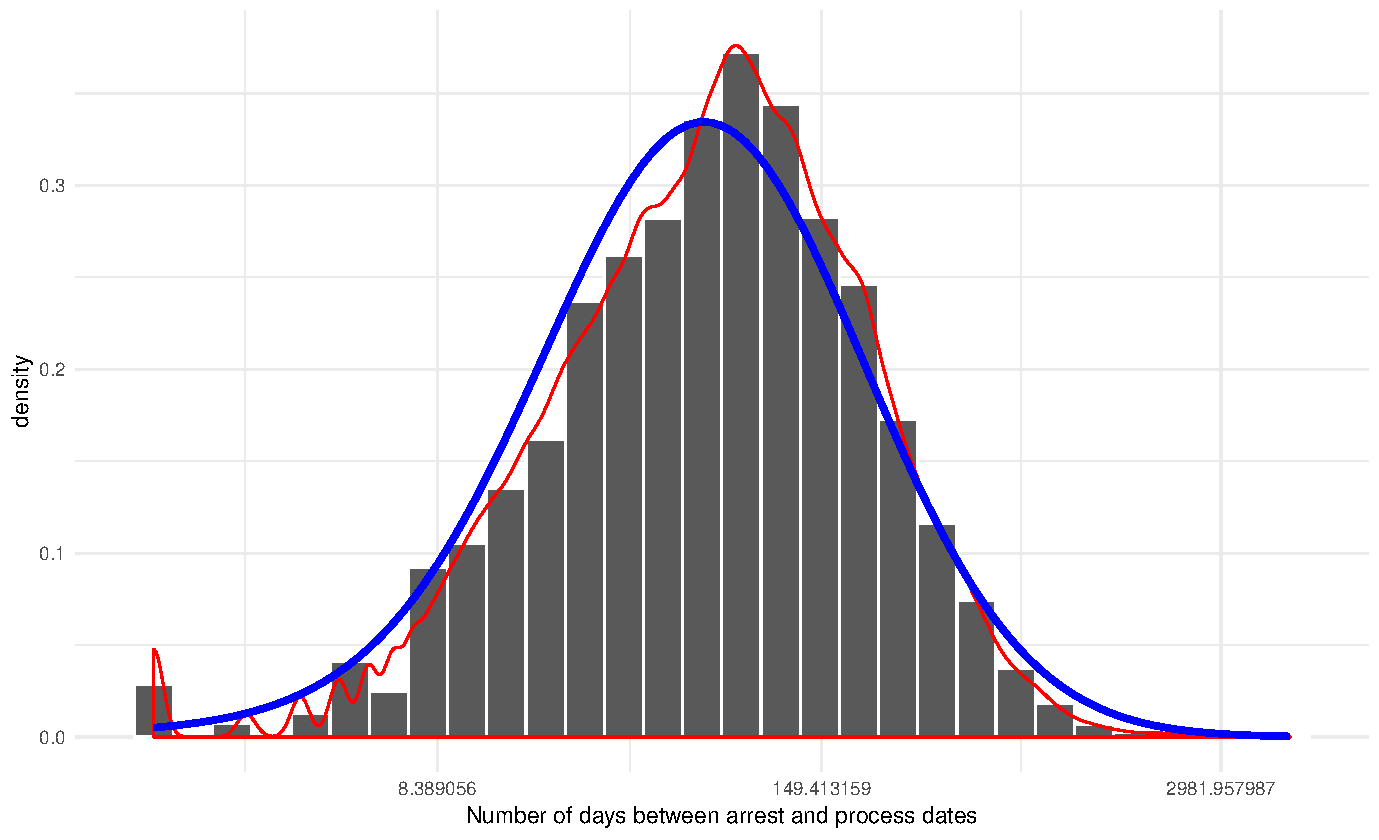
\includegraphics[width=\textwidth]{plots/imputing_arrest_date/simple_lm_hist.pdf}
\label{fig:simple_lm_hist}
\begin{minipage}{0.92\textwidth}
\footnotesize
\emph{Notes:} The x-axis is shown on  $\log(1 + x)$ scale.
\end{minipage}

\end{figure}

To address this problem, we model the zero and positive values separately in a two-stage process 
%by first predicting if a the number of days is zero and then fitting log-normal regression to the positive date. 
using a method described in \citet[p. 537-538]{gelman_data_2006}. 
Let $y$ be the number of days between arrest of an individual and his or her trial and $X$ be set of dummy variables indicating the year of trial. We also define $I^y$ as an indicator variable that equals 1 if $y > 0$ and 0 otherwise and  $y^{\text{pos}}$ to be only positive values of $y$ (i.e. $y^{\text{pos}} = y$ if   $y > 0$).  In the first stage, we predict $I^y$  using logistic regression
\begin{equation}
\Pr\left( I_i^y = 1 \right)  = \text{logit}^{-1} \left(X_i \alpha \right).
\end{equation}
In the second stage, simple log-linear regression is applied to predict only the positive values $y^{\text{pos}}$
\begin{equation}
\log\left(y_i^{\text{pos}}\right) \sim \text{N} \left(X_i \beta, \sigma \right).
\end{equation}
We then fit the first model to the data where the exact dates of both arrest and trial are available and the second model to the subset of the same  data for which $y > 0$.
The results of both of these models are provided in the table \ref{tab:date_imp_results} in the appendix. The years of trial appear to be important predictors both in the first stage and even more in the second stage. 
However, the unexplained variance is still high making up about 76\% of the total variability in the dependent variable in the second model. 

%After  these models are fitted to the data with non-missing date of arrest and year of process,
We  proceed to apply the fitted models to the missing data to get the predicted probability of $y$  being positive and the mean value of $y$ if it is positive. For each observation with missing date of arrest $X_i$, we then randomly draw from the Bernoulli distribution with  $\text{logit}^{-1} \left(X_i \hat\alpha \right)$ as its parameter to obtain $\hat I_i^y$. We also draw from the normal distribution with mean $X_i \hat\beta$ and exponentiate the result to get $\hat y_i^{\text{pos}}$. Finally, the predicted number of days is calculated simply as $\hat y_i = \hat I_i^y \cdot \hat y_i^{\text{pos}}$. 

The histogram of the imputed values is provided in the figure \ref{fig:mixed_model_preds_hist} in the appendix. 
The resulting distribution  highly resembles the distribution  in the figure \ref{fig:simple_lm_hist} including the fraction of zero values indicating our model captures the actual data fairly well. 

Nevertheless,  one issue is that for significant number of observations we do not have the exact date of trial but only year. In particular, 
while the year of trial is recorded for all 903 455 observations where the date of arrest is to be imputed, the month of trial is missing for 369 393 of them and the day for 390 174. 
To fill in the missing month, we take a random sample from all months with probability equal to the relative frequency of the months of trial in the non-missing data between the years 1921 to 1960. 
Even simpler method is used to impute the missing days where we just randomly choose a day within given month with uniform probability.\footnote{Every date, however, has to be consistent with the calendar. This means that for January we take a sample of numbers from 1 to 31, for February from 1 to 28 and so on. } 
The imputed months and days of the trials are therefore only weakly informed guesses, nevertheless they enable us to carry on with the analysis. 

%Once we have completed the above steps, 
The final step is to calculate the imputed date of arrest by subtracting the predicted number of days from the date of process (i.e. we go back in time by given number of days). Since we conduct the analysis with annual observations, we ignore predicted month and day of arrests  keep only information on year. The number of arrests for each ethnicity by year (including the imputed years) is then counted for the period from 1921 to 1960 which forms our final dataset. 

The resulting time series of all arrests with imputed years is plotted in the figure \ref{fig:date_imputation_line} in the appendix. Arrests with imputed dates seem to follow  similar trends with the labeled data  although there is slight divergence at the beginning and end of the series and in the 1930s.
%involves only counting back 
%we have the exact date of process and the predicted 
%for the subset of the data where the date of arrest is to be imputed, 369 393 observations lack the month of the process and 390 174 miss the day out of the total 903 455 (all have year). 